
%
% a front end for the draft
%
% This version is actually what I gave to my committee
% and published as a tech report.
% IMHO, the report style is much better for human consumption
% than the required thesis style.
%    -johnh, 12-Jan-96
%

\newif\ifissubmit
\issubmitfalse

\newif\ifisdraft
\isdrafttrue

% \documentclass[PhD,single,twoside]{uclathes}
\documentclass[twocolumn,twoside]{book}
\usepackage{times}

%%%%%%%%%%%%%%%%%%%%%%%%%%%%%%%%%%%%%%%%%%%%%%%%%%%%%%%%%%%%%%%%%%%%%%
%
% format hacking:
%

\makeatletter

  %
  % get the thesis title page format
  %
  \input{uclathma.clo}
  \input{uclathti.clo}

  %
  % sectiion titles
  %
  \renewcommand\section{\@startsection {section}{1}{\z@}%
                                     {-3.5ex \@plus -1ex \@minus -.2ex}%
                                     {2.3ex \@plus.2ex}%
                                     {\reset@font\Large\bfseries\nohyphenation}}
  \renewcommand\subsection{\@startsection{subsection}{2}{\z@}%
                                       {-3.25ex\@plus -1ex \@minus -.2ex}%
                                       {1.5ex \@plus .2ex}%
                                       {\reset@font\large\bfseries\nohyphenation}}
  \renewcommand\subsubsection{\@startsection{subsubsection}{3}{\z@}%
                                       {-3.25ex\@plus -1ex \@minus -.2ex}%
                                       {1.5ex \@plus .2ex}%
                                       {\reset@font\normalsize\bfseries\nohyphenation}}
  \renewcommand\paragraph{\@startsection{paragraph}{4}{\z@}%
                                      {3.25ex \@plus1ex \@minus.2ex}%
                                      {-1em}%
                                      {\reset@font\normalsize\bfseries\nohyphenation}}
  \renewcommand\subparagraph{\@startsection{subparagraph}{5}{\parindent}%
                                         {3.25ex \@plus1ex \@minus .2ex}%
                                         {-1em}%
                                        {\reset@font\normalsize\bfseries\nohyphenation}}

  %
  % Steal the bibliography from uclathes so it's a real chapter.
  %
  \def\thebibliography#1{\chapter*{References\markboth
    {REFERENCES}{REFERENCES}}
    \addcontentsline{toc}{chapter}{References}
    \renewcommand\baselinestretch{1}
    \@normalsize
    \list{[\arabic{enumi}]}{\settowidth\labelwidth{[#1]}\leftmargin\labelwidth
      \advance\leftmargin\labelsep
      \usecounter{enumi}}
      \def\newblock{\hskip .11em plus .33em minus -.07em}
      \sloppy
      \sfcode`\.=1000\relax}
  
  \def\endthebibliography{\renewcommand\baselinestretch{\@spacing}\@normalsize\endlist}
  
  %
  % margin hacking
  %
  %
  % First get rid of driver margins.
  \setlength{\voffset}{-1in}
  \setlength{\hoffset}{-1in}
  % Set column width and gutter
  \setlength{\textheight}{8.5in}
  % Top and bottom margins.
  \setlength{\topmargin}{0.75in}
  \setlength{\headheight}{12\p@}
  \setlength{\headsep}{0.25in}
  \setlength{\footskip}{0.35in}
  % Left and right margins.
  \setlength{\evensidemargin}{0.80in}
  \setlength{\oddsidemargin}{1.25in}
  % width
  \setlength{\textwidth}{6.45in}
  \setlength{\columnsep}{0.25in}


\makeatother



%
% main.tex
% Copyright (C) 1995 by John Heidemann, <johnh@isi.edu>.
% $Id: demo2big.tex,v 1.2 1996/01/16 18:57:04 johnh Exp $
%


%
% thesis_macros
% Copyright (C) 1995 by John Heidemann, <johnh@isi.edu>
%

% \RequirePackage{johnh_general}

\RequirePackage{ifthen}

% \def\epsfreduction{0.667}
\def\epsfgraphreduction{0.9}

\newcommand\comment[1]{{[\sffamily #1]}}

%
% TeX seems to want to indent after chapters,
% although it shouldn't.  Rather than argue
% with it, I work around it manually by putting this
% hack in the right places:
\newcommand{\noindenthack}{\noindent}


\newcommand{\fwling}{featherweight layering}
\newcommand{\fwls}{featherweight layers}
\newcommand{\fwl}{featherweight layer}

\newcommand{\Fwling}{Featherweight layering}
\newcommand{\Fwls}{Featherweight layers}
\newcommand{\Fwl}{Featherweight layer}

\newcommand{\FwLing}{Featherweight Layering}
\newcommand{\FwLs}{Featherweight Layers}
\newcommand{\FwL}{Featherweight Layer}

\newcommand{\xvop}[2]{{\scomputer {{#1}\_{#2}}}}
\newcommand{\vop}[1]{\xvop{vop}{#1}}

\newcommand{\usec}{$\mu$seconds}
\newcommand{\unix}{Unix}

\newcommand{\dotdot}{\scomputer{..}}

\newenvironment{mycode}%
	{\small
	}{%
	}

\newcommand{\mylangle}{\langle}
\newcommand{\myrangle}{\rangle}
\newcommand{\myrightarrow}{\rightarrow}


%
% Sizes of various things:
%
  \newcommand{\tablesize}{\normalsize}
  \newcommand{\computertablesize}{\small}
  \newcommand{\bibliographysize}{\normalsize}

  %
  % Another space-saver:  shrink the figures and graphs.
  %
 \def\epsfreduction{0.85}
 \def\epsfgraphreduction{0.9}   % should be left at 0.9 with two-column text
% \def\epsfsize#1#2{\epsfreduction#1}

%\newcommand{\appendixnumbering}{
%	\renewcommand{\thechapter}{\Alph{chapter}}
%	\setcounter{chapter}{0}
%	}

\newenvironment{functions}%
	{\begin{description}}%
	{\end{description}}

\makeatletter
  \newcommand{\SubmitSingleSpace}{
    \ifissubmit
      \renewcommand\baselinestretch{\@singlespacing}\@normalsize
    \fi
  }
  \newcommand{\SubmitDoubleSpace}{
    \ifissubmit
      \renewcommand\baselinestretch{\@doublespacing}\@normalsize
    \fi
  }
\makeatother


\iffalse
Figure drawing style guide:

layer labels:
	helvetica 12pt bold
	(short acronyms) helvetica 14pt bold

spacing:  8 pixels
each layers will be 3 high and 7 or 7.5 wide

or spacing: 8 pts
each layer will be 4 high and 10 wide

boxes and vnode links are line #2
\fi



\begin{document}


%
% Title pages of the thing
% Copyright (C) 1995 by John Heidemann, <johnh@isi.edu>.
%



\title{Stackable Design of File Systems}
\author{John~Shelby Heidemann}


\department{Computer Science}
\degreemonth{September}
\degreeyear{1995}

\chair{Gerald~J.~Popek}
\chair{D.~Stott Parker}
\member{Richard~Muntz}
\member{Rajive~L.~Bagrodia}
\member{Kirby~A.~Baker}

\dedication{\textsl{Are you dedicated?}}

\acknowledgments{
Ack!  P'tui.
}

%%%%%%%%%%%%%%%%%%%%%%%%%%%%%%%%%%%%%%%%%%%%%%%%%%%%%%%%%%%%%%%%%%%%%%
%
% vita
%
\vitaitem{1968}{B.S., Computer Science, Caribou University}
\vitaitem{etc.}{etc.}
\vitaitem{1995}{Graduated, UCLA}

%%%%%%%%%%%%%%%%%%%%%%%%%%%%%%%%%%%%%%%%%%%%%%%%%%%%%%%%%%%%%%%%%%%%%%
%
% publications
%

\publication{
	Richard~G.\ Guy, John~S.\ Heidemann, Wai Mak, Thomas~W.\ Page,~Jr.,\ 
	  Gerald~J.\ Popek, and Dieter Rothmeier.
	Implementation of the Ficus
	  replicated file system.
	In \emph{USENIX Conference Proceedings}, pages
	  63--71.
	USENIX, June 1990.
}

\publication{
	etc.
}




%%%%%%%%%%%%%%%%%%%%%%%%%%%%%%%%%%%%%%%%%%%%%%%%%%%%%%%%%%%%%%%%%%%%%%


Dark matter makes up most of the mass in the Universe, and yet its particle properties remain unknown. As dark matter drives structure formation in the Universe, clues regarding the particle nature of dark matter are imprinted in the abundance and density profiles of dark matter halos. Measurements of the halo mass function and the concentrations of individual dark matter halos, particularly on sub-galactic scales, can therefore be cast as direct constraints on the particle nature of dark matter.

Strong gravitational lensing by galaxies offers a unique probe of dark matter structure in the Universe across cosmological distance. By coupling directly to gravity, lensing probes structure without relying on luminous matter as a tracer of the underlying dark matter. The direct gravitatioanl coupling also extends the reach of lensing probes below $10^8$ solar masses, where halos are mostly devoid of stars and gas, and where various dark matter theories make divergent predictions for the halo mass function and the mass-concentration relation of halos. 

In this dissertation, I present the development of a forward modeling framework to constrain any model based on dark matter theory, provided the model makes predictions for the form of the halo mass function and the density profile of individual dark matter halos. The formalism I present handles the marginalization over nuisance parameters, including the mass profile of the main deflector and finite source effects, in a fully Bayesian framework, and accounts for both subhalos associated with the main deflector and field halos along the line of sight. 

Using the framework I developed, my thesis presents an unprecedented constraint on the free-streaming length of dark matter that corresponds to a lower limit of $5.2 \rm{keV}$ on the mass of a thermal relic dark matter particle. In addition, I present the first measurement of the mass-concentration relation of Cold Dark Matter halos on sub-galactic scales across cosmological distance. 

%
% I built a custom title page to do what I want.  So sue me.
% NEEDSWORK:  I had to copy some stuff from uclathti.sty.
%
\makeatletter
  \newcommand{\CustomTitlePage}{
    \begin{titlepage}
      \ColumnSave
      \vspace*{1.5in}   % a hacky way to center.  TeX didn't like \vfill.
      \begin{center}
  
      {\bfseries\huge \@title} \\
      \vskip 48pt plus0pt minus18pt
  
      {\large \@author} \\
      \vskip 12pt plus0pt minus3pt
      {\large University of California, Los Angeles} \\
      \vskip 6pt plus0pt minus2pt
      {\large \@degreemonth, \@degreeyear} \\
      \vskip 48pt plus0pt minus18pt
  
      \normalsize A \@thesisname\
      submitted in partial satisfaction \\
      of the requirements for the degree \\
      \@degreename\if@department\ in \@department \fi\\
      \vskip 24pt plus0pt minus6pt

      \normalsize
	UCLA Computer Science Department \\
	Technical Report UCLA-CSD-950032 \\
      \vskip 24pt plus0pt minus6pt

      \textbf{Thesis committee:} \\
      \ifnum\c@chairs<1
        \typeout{No committee chair.}
      \else\ifnum\c@chairs<2
        \@chairA, chair \\
      \else\ifnum\c@chairs<3
        \@chairA, co-chair \\
        \@chairB, co-chair \\
      \else\ifnum\c@chairs<4
        \@chairA, co-chair \\
        \@chairB, co-chair \\
        \@chairC, co-chair \\
      \fi\fi\fi\fi
      \ifnum\c@members<1 \typeout{No non-chair committee members.}\fi
      \ifnum\c@members>0 \@memberA \\ \fi
      \ifnum\c@members>1 \@memberB \\ \fi
      \ifnum\c@members>2 \@memberC \\ \fi
      \ifnum\c@members>3 \@memberD \\ \fi
      \ifnum\c@members>4 \@memberE \\ \fi
      \ifnum\c@members>5 \@memberF \\ \fi

      \end{center}
    \end{titlepage}
  }

  \newcommand{\CustomAcknowledgePage}{
  \chapter*{Acknowledgments}

  \@acknowledgments
  }
\makeatother

\ifissubmit
  \makeintropages
\else
  \makeatletter
    \pagenumbering{roman}
    \CustomTitlePage
    \@makecopyrightpage
    \@makededication
    \tableofcontents
    \listoffigures
    \listoftables
    \cleardoublepage
    \@makeabstractpage{1.0}
    \CustomAcknowledgePage
%    \@makevitapage

    \cleardoublepage
    \pagestyle{headings}
    \pagenumbering{arabic}
    \setcounter{page}{1}
  \makeatother
\fi


% LocalWords:  Stott Muntz Ted Yu Wu Michial Gunter Stovall Salomone Louie Qian
% LocalWords:  Qin Weidner McKusick Pendry Minshall kitrace Ousterhout CSD ftp
% LocalWords:  Administrativia csd ps HyperCard Yarvis Alexy Rudenko pt Los co
% LocalWords:  degreemonth degreeyear thesisname degreename chairA chairB roman
% LocalWords:  chairC memberA memberB memberC memberD memberE memberF arabic
% LocalWords:  makecopyrightpage makededication makeabstractpage Monique http
% LocalWords:  Bennarosh www html


%
% introduction.tex
% Copyright (C) 1995 by John Heidemann, <johnh@isi.edu>.
% $Id: demo2int.tex,v 1.1 1996/01/12 18:13:58 johnh Exp $
%

\chapter{Introduction}

\indent All is not well in cosmology. Dark matter, an entity of unknown origin and particle nature, makes up approximately $80\%$ of the mass in the Universe. Gravity mediates the only known interaction between us and this mysterious substance. Through gravity, dark matter pulls the strings of cosmic structure formation, explaining the formation and evolution of galaxies like the Milky Way. Through gravity, dark matter also bends the path of light. 

Approximately 9 billion years ago, four photons were ejected from the quasar WFI 2033-4723. Left to fly freely, a distance of roughly $100,000$ light years would separate them at the present time; instead, we find the photons collected today on the primary mirror of the Hubble Space Telescope. The gravitational field of a massive galaxy and its surrounding dark matter, precisely aligned between us and WFI 2033-4723, intervened to deflect light emitted from the distant quasar. The warping of space caused by the foreground galaxy is so extreme that several different paths connect Hubble with the background source, creating multiple images of the quasar at various positions on the sky. This phenomenon is referred to as strong gravitational lensing. Figure \ref{fig:lens2033} shows six examples of quadruple-image strong lenses, or \textit{quads}, including the system WFI 2033-4723.

The positions and magnifications of the multiple images in quads encode information regarding the abundance and density profiles of dark matter halos between us and the lensed background source. If the reigning cosmological theory of Cold Dark Matter (CDM) is correct, countless gravitationally-bound structures, or \textit{halos}, litter the cosmos and produce gravitational lensing effects. A positive detection of these otherwise-undetectable dark matter halos through lensing would confirm a central prediction of CDM. Alternatively, some models based on dark matter theory predict that halos do not exist below a certain mass scale, which itself depends on the formation mechanism and mass of the dark matter particle(s). A non-detection of halos below a certain mass scale would therefore potentially overthrow entire classes of models, including CDM, that predict a plethora of dark matter structure in the Universe. Either result would bring us one step closer towards understanding the nature of dark matter, and resolving one of the most confounding problems facing modern cosmology. 

\begin{figure*}
	\centering
	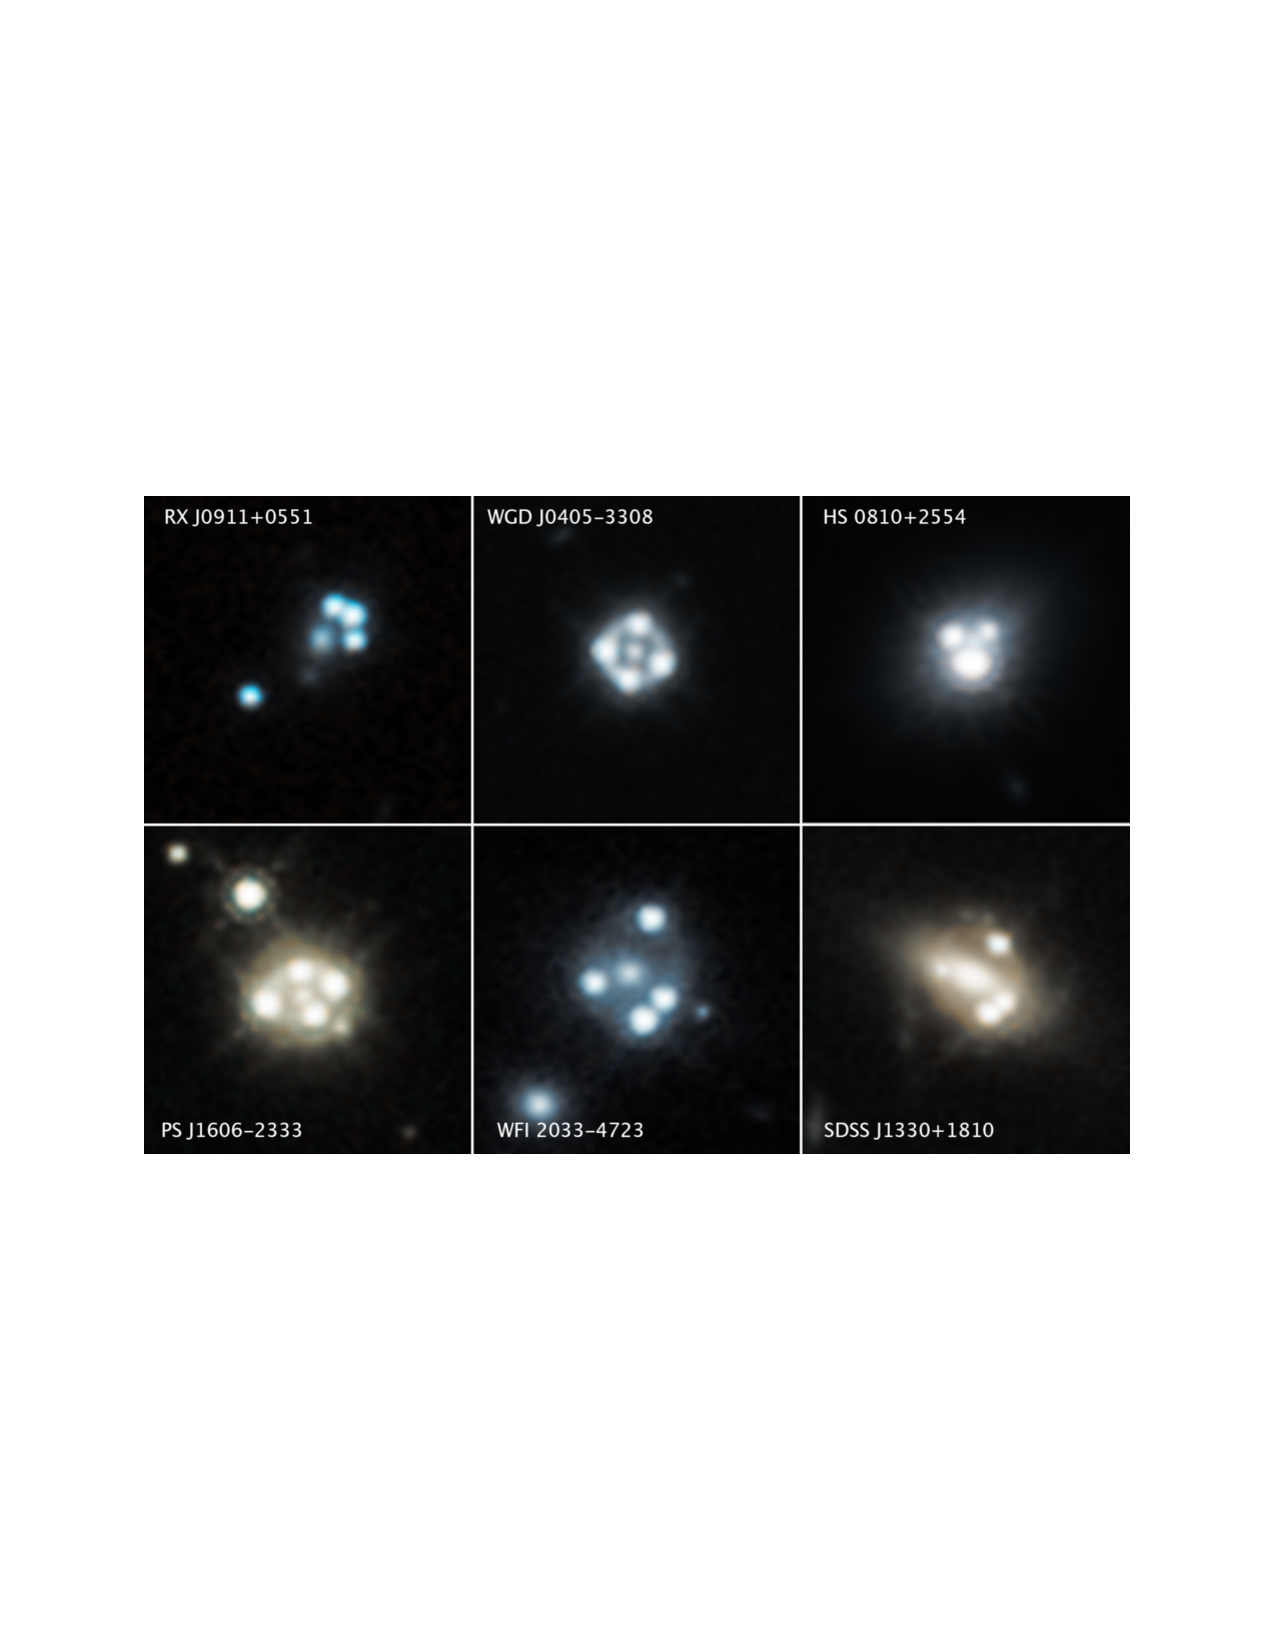
\includegraphics[clip,trim=2.5cm 8cm 2.5cm
	8.5cm,width=.95\textwidth,keepaspectratio]{./figures_introduction/lenses.pdf}
	\caption[Six images of strong gravitational lenses]{\label{fig:lens2033} Six quadruple-image strong gravitational lens systems imaged by the Hubble Space Telescope \citep{Nierenberg++19}. The main lensing galaxy is visible as the faint object encircled by four highly-magnified images of a background quasar. Image credit: NASA, ESA, A. Nierenberg (JPL) and T. Treu (UCLA)}
\end{figure*}	
In this dissertation, I describe research that constrains particle theories of dark matter with strong gravitational lensing. The following sections of this introduction set the stage for Chapters 2-6, which describe the development and implementation of a technique to constrain any dark matter model using the image magnifications from a sample of quads. Section 1.1 begins with a review of how the particle nature of dark matter drives structure formation in the Universe, and what aspects of structure formation lensing can constrain. Next, I review the basic theory connecting dark matter structure to lensing observables. 

\section{Structure formation and dark matter physics}
\indent An initially diffuse field of dark matter particles will collapse into gravitationally-bound halos through a mechanism called `violent relaxation' \citep{LyndenBell67}. The halo mass function, or the number of halos per unit mass, encodes information about when the first dark matter halos collapsed in the early Universe. Similarly, the density profiles of individual halos as a function of mass, the mass-concentration relation, depends on the hierarchical assembly of dark matter halos through cosmic time, and the shape of the primordial matter power spectrum that seeded the growth of structure. The particle nature of dark matter affects both the initial matter power spectrum and the growth of density fluctuations initialized at early times, imprinting clues regarding the particle nature of dark matter in the large and small-scale structure of the Universe. 

As a concrete example, consider two competing classes of dark matter models: Cold, and Warm Dark Matter (CDM and WDM, respectively). A quantity called the free-streaming length $\lambda_{\rm{FS}}$ distinguishes these two models. By definition, free-streaming effects are negligible in CDM. In WDM scenarios, diffusion of dark matter particles out of potential wells initialized in the early Universe wipes out small-scale density fluctuations. This diffusion process transforms a density field initialized with a scale-free power spectrum $P\left(k\right) \propto k^{n}$ into a density field with a power spectrum truncated at a scale $k_{\rm{FS}} = \frac{2 \pi}{\lambda_{FS}}$. The characteristic length scale $\lambda_{\rm{FS}}$ can be approximated as the comoving distance a particle could have traveled before structure begins growing in earnest around the time of matter-radiation equality $t_{\rm{EQ}}$ \citep{Schneider++12} 
\begin{figure}
	\centering
	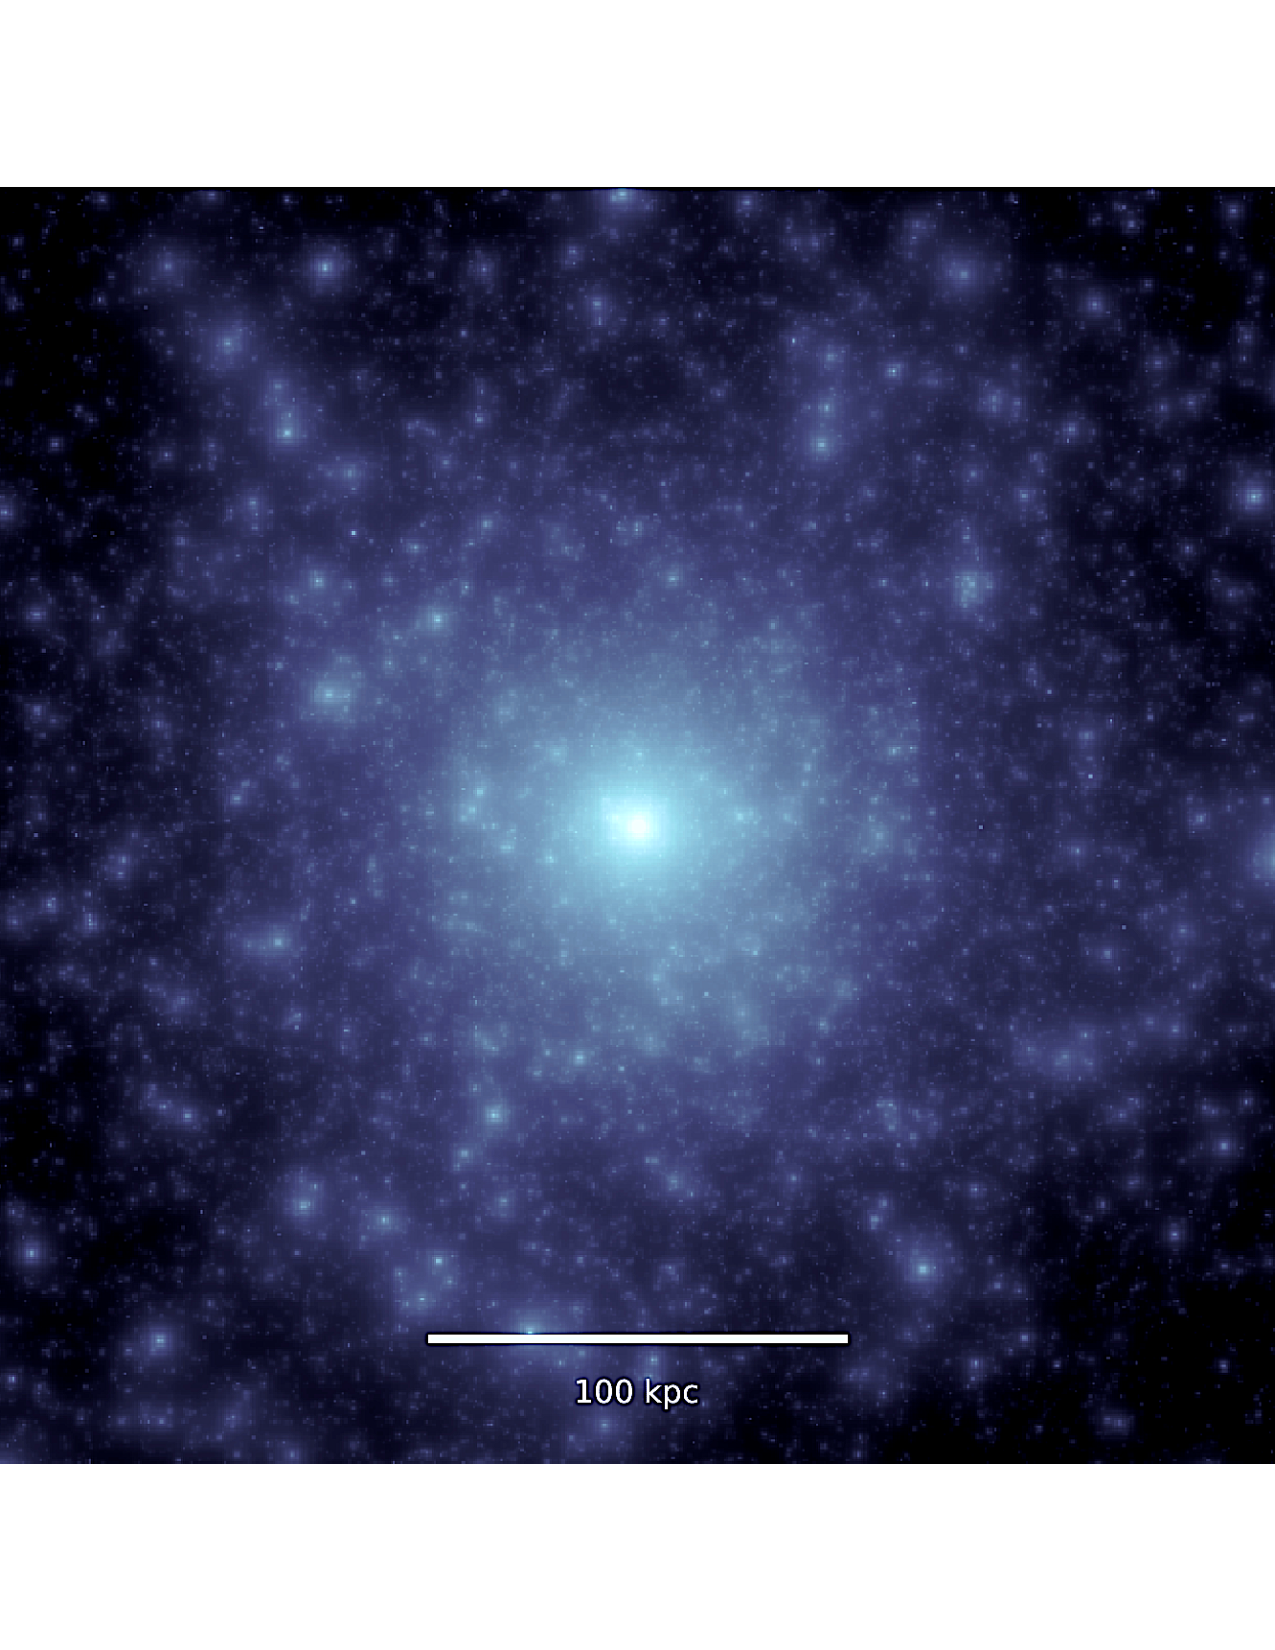
\includegraphics[clip,trim=0cm 0cm 0cm
	0cm,width=.49\textwidth,keepaspectratio]{./figures_introduction/CDMscreenshot_edited.pdf}
	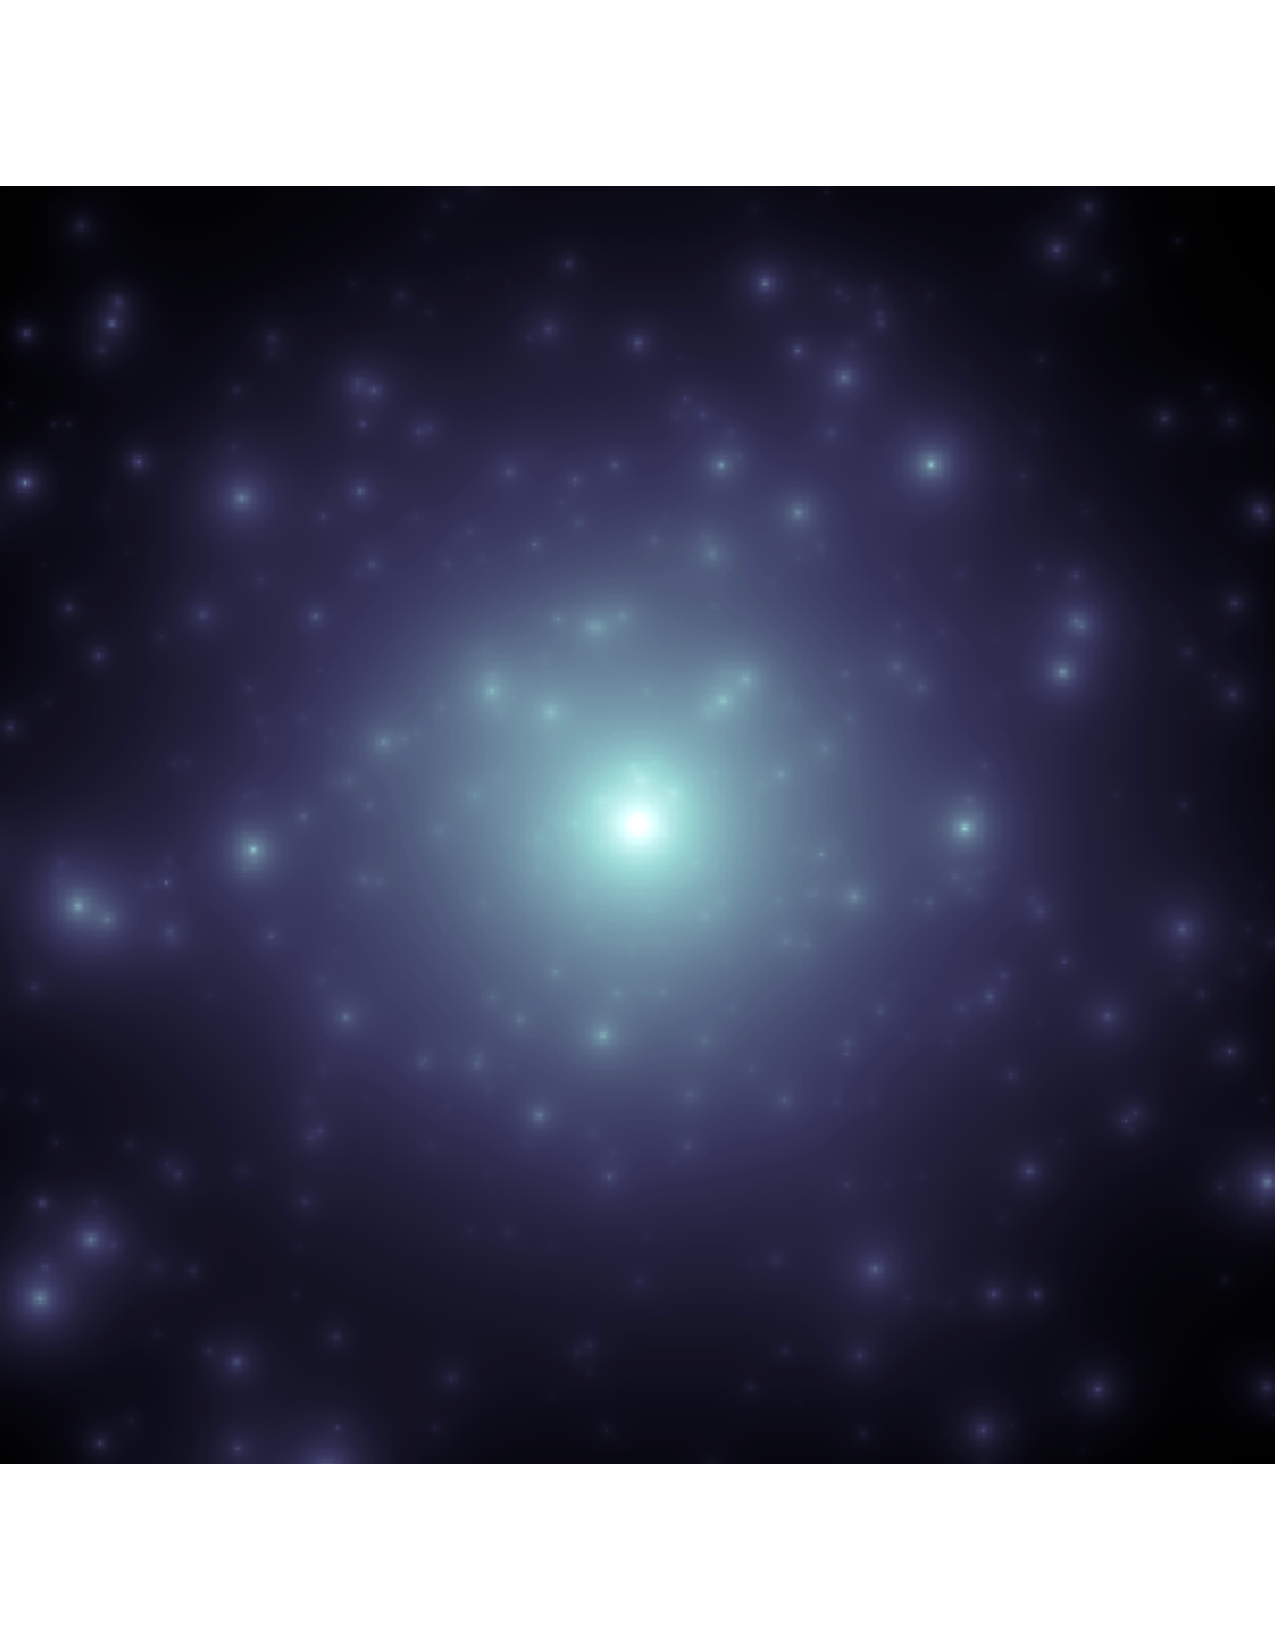
\includegraphics[clip,trim=0cm 0cm 0cm
	0cm,width=.49\textwidth,keepaspectratio]{./figures_introduction/WDMrealization_nobar.pdf}
	\caption[CDM and WDM subhalo populations]{\label{fig:wdmrealization} {\bf{Left:}} A realization of CDM substructure, with a scale-free subhalo mass function. {\bf{Right:}} A realization of WDM substructure corresponding to a $3.3 \rm{keV}$ thermal relic dark matter particle, which produces a turnover in the halo mass function around $10^8$ solar masses. }
\end{figure}

\begin{equation}
\label{eqn:freestreaming}
\lambda_{FS} \approx \int_{0}^{t_{\rm{NR}}} \frac{c dt}{a\left(t\right)} +  \int_{t_{\rm{NR}}}^{t_{\rm{EQ}}} \frac{v\left(t\right) dt}{a\left(t\right)} \approx r_{H}\left(t_{\rm{NR}}\right) \left(1 +\frac{1}{2} \log \frac{t_{\rm{EQ}}}{t_{\rm{NR}}} \right),
\end{equation}
where the particle has speed $c$ before becoming non-relativistic at time $t_{NR}$, $r_H \left(t_{\rm{NR}}\right)$ is the comoving horizon size at $t_{\rm{NR}}$, $a\left(t\right)$ is the cosmological scale factor, and $v\left(t\right)$ represents the average velocity distribution of the dark matter particles\footnote{This expression assumes that the particles become non-relativistic before $t_{\rm{EQ}}$, and uses the fact that $a\left(t\right)\propto t^{\frac{1}{2}}$ before $t_{\rm{EQ}}$.}. 

The effects of free-streaming manifest in structure formation in two ways: First, erasing small-scale power at early times eliminates the small-scale density fluctuations in the primordial matter density field that would eventually collapse into the smallest dark matter halos. This suppression of small-scale power results in a turnover in the halo mass function at a certain mass scale that is proportional to the $k_{\rm{FS}}^{-3}$ \citep{AvilaReese++01,Schneider++12,Lovell++14}. Second, because low-mass halos collapse first in hierarchical structure formation scenarios, eliminating the smallest halos delays the onset of structure formation. As the central density profile of a dark matter halo reflects the background density of the Universe at the time of collapse, delaying structure formation suppresses the central density of dark matter halos. Mergers between low-mass halos into larger halos propagate these effects to larger halo masses, affecting structures over an order of magnitude in mass above the scales that are directly impacted by free-streaming effects \citep{Navarro++96,Bose++16}. These structure formation arguments apply to both isolated halos in the field, and subhalos of the $10^{13}$ solar mass host dark matter halos that contain early-type galaxies typically acting as strong lenses \citep{Gavazzi++07}. The left and right panels of Figure \ref{fig:wdmrealization} show examples of CDM and WDM subhalo populations, respectively. 

The dependence of $\lambda_{FS}$ on features such as $t_{NR}$ and $v\left(t\right)$ links the free-streaming length of the dark matter to the formation mechanism and velocity distribution of the dark matter particle(s). As the halo mass function and mass-concentration relation depend on the free-streaming length, it follows that constraining the halo mass function and halo density profiles can be cast as a constraint on fundamental dark matter physics determining $t_{NR}$ and $v\left(t\right)$. Notice, however, that none of the previous discussion depends on a particular choice dark matter particle. We can simultaneously rule out neutrinos, thermal relics with mass $< 2 \rm{keV}$, and sterile neutrinos produced via Higgs decay with a mass of $7 \rm{keV}$ \citep{Viel13,AbazaijanKusenko19} making up 100$\%$ of the dark matter, as the free-streaming lengths corresponding to each these models precludes the formation of galaxies such as the Milky Way. Properties like the free-streaming length can be computed for practically any model in the literature, illustrating the broad scope and power of structure formation arguments. 

In order to employ structure formation arguments, one requires a method to detect, and measure the mass of, dark matter halos. One approach uses the fact that galaxies are believed to reside inside dark matter halos; luminous structures, such as galaxies, therefore trace the underlying dark matter. Unfortunately, the approach of using luminous matter as a proxy for invisible halos becomes increasingly difficult below $10^9$ solar masses, as not every halo on these scales hosts a visible galaxy. Moreover, uncertainties that stem from astrophysics on sub-galactic scales that determine how one assigns a dark matter halo mass to an observed galaxy can sometimes be larger that the differences between predictions from the dark matter models of interest \citep{Nierenberg++16}. While recent advances in this field make considerable progress towards appropriately dealing with these complications \citep{Nadler++19}, the systematic uncertainties persist. A second technique to probe small-scale structure in the Universe relies on the flux power spectrum of the Lyman-$\alpha$ forest at $z \sim 5$, which under certain assumptions can be used as a proxy for the matter power spectrum \citep{Viel13,Irsic++17}. The promise of this method must be weighed against the systematic uncertainties associated with thermodynamic processes relevant to the Lyman-$\alpha$ forest, which can mimic the suppression of small-scale power predicted in WDM scenarios \citep{Garzilli++19}. 

Strong gravitational lensing by galaxies offers an alternative, more direct probe of dark matter structure on scales below $10^8$ solar masses. Lensing couples only to gravity, and therefore circumvents the challenges associated with using baryonic matter to trace the underlying dark matter. In the next section, I review the formalism connecting lensing observables to populations of dark matter halos along the entire line of sight from the observer to the source. 

\section{Strong lensing signatures of dark matter halos}
\indent General relativity relates the deflection angle of a light ray to the mass distribution of a massive structure, dark or luminous. When the distances scales between the observer, lens, and source are much greater than the physical extent of the lensing mass distribution, the effect of a massive deflector can be approximated as a single sharp deflection in the plane of the lens, the `thin lens' approximation. Defining $\Sigma\left(\vec{\xi}\right)$ as the projection of a deflector's three dimensional density profile onto the plane of the lens at the coordinate $\vec{\xi}$, the deflection angle is given by \citep{BlandfordNarayan86}
\begin{equation}
\label{eqn:defangle}
\vec{\alpha}\left(\vec{\xi}\right) = \frac{4G }{c^2} \int \frac{\left(\vec{\xi} - \vec{\xi^{\prime}}\right) \Sigma\left(\vec{\xi^{\prime}}\right)}{| \vec{\xi} - \vec{\xi^{\prime}}|^2} d^2 \xi^{\prime}. 
\end{equation}
For multiple deflectors in a single lens plane, the cumulative effect is a linear superposition of their individual deflection angles $\vec{\alpha}$. 

A strong lens system will include both subhalos associated with the host dark matter halo of the lensing galaxy, and field halos distributed along the entire line of sight. Incorporating field halos requires the multi-plane ray tracing equation, which maps an angular coordinate on the sky $\vec{\theta_1}$ to an angular coordinate on the source plane $\vec{\theta_s}$. The ray tracing equation that determines where images appear to the observer is given by \citep{BlandfordNarayan86}
\begin{equation}
\label{eqn:raytracingintro}
\vec{\theta_s} = \vec{\theta_1} - \frac{1}{D_{\rm{s}}} \sum_{i=1}^{s-1} D_{\rm{is}}{\vec{\alpha_{\rm{i}}}} \left(D_{\rm{i}} \vec{\theta_{\rm{i}}}\right),
\end{equation} 
where the net deflection angle from all halos at the $i$th lens plane can be computed with Equation \ref{eqn:defangle}, $D_{\rm{ij}}$ is the angular diameter distance from the $i$th lens plane to the $j$th, and subscript $s$ identifies the source plane. Equation \ref{eqn:raytracingintro} is a recursive equation for the position of deflected light rays at each lens plane. It describes a physical process similar to viewing an image through multiple magnifying glasses in series, coupling deflections produced by objects at different distances. 

As gravitational lensing conserves surface brightness \citep{MisnerThorneWheeler}, the (de)magnification of the lensed images is proportional to the ratio of areas in the image and source planes. This factor is computed from the inverse determinant of the jacobian $\left(\det \frac{\partial \vec{\theta_s}}{\partial \vec{\theta_1}}\right)^{-1}$. While the full expression for the lensing jacobian in the general multi-plane framework (see \citet{BlandfordNarayan86}) is long and not particularly illuminating, the key point is that the magnification of an image depends non-linearly on derivatives of the lensing deflection angle. Image magnifications are therefore highly localized probes of the mass distribution along the line of sight to strong lenses. While the exact level of perturbation to an image magnification depends on the size of the background source, the mass of the halo, and the position of the image relative to the critical curve, a dark matter halo as small as $10^7 M_{\odot}$ near a lensed image can induce measurable perturbations on image magnifications for background sources of size $O\left(10\right)$ pc. 

The idea that dark matter halos frequently perturb image magnifications was first put forward in 1997 \citep{MaoSchneider98}. Since that time, authors have attributed lensing `flux anomalies', or the consistent failure of smoothly-parameterized mass distributions to reproduce the magnifications ratios observed in quad lens systems\footnote{Since the intrinsic brightness of the source is unknown, the observable quantity is the magnification ratio, rather than the magnification itself.}, to the presence of substructure in the lens system \citep{Metcalf++02,D+K02,FadleyKeeton12,Xu++12,Nierenberg++14,Nierenberg++19}. Early studies of strong lensing flux anomalies (e.g. \citet{D+K02}) relied on lensed radio emission from the background quasar. This technique has drawbacks that are remedied by the advent of nuclear narrow-line emission from the background quasar as probe of substructure, a method first proposed by \citet{MoustakasMetcalf02}, and subsequently implemented by \citet{Sugai++07,Nierenberg++14,Nierenberg++17,Nierenberg++19}. The use of lensed narrow-line emission has two advantages: First, the nuclear narrow-line region is spatially extended by $\sim 50$pc \citep{MullerSanchez++11}, preventing contamination from microlensing and variability in background source brightness\footnote{The light crossing time of the narrow-line region washes out the small-scale variability in the light curve of the background source.}, processes that considerably inflate uncertainties in radio flux ratios. Second, narrow-line emission is present in the spectrum of virtually every quasar, expanding the sample size of available lens systems. Recently, the sample size of strong lens systems with measured narrow-line flux ratios increased by nearly a factor of four \citep{Nierenberg++19}. 

During my PhD, I developed a flexible and powerful Bayesian inference framework that takes full advantage of flux ratios measured using nuclear narrow-line emission to constrain any dark matter model, provided the model predicts the shape of the halo mass function, and the density profile of individual halos. The methods I developed improve over previous work in two key ways: First, they account for halos along the line of sight to strong lenses, which can sometimes outnumber the subhalos associated with the main deflector. Second, the method naturally accommodates spatially extended background sources, which affect the sensitivity of lensing observables to dark matter halos. The tools I developed delivered one of the tightest constraints on the free-streaming length of dark matter to date (see Chapter 5), independent of and more stringent than those obtained from the Lyman-$\alpha$ forest \citep{Viel13}, and the first observational constraint on the mass-concentration relation of CDM halos on sub-galactic scales across cosmological distance (see Chapter 6). 

This dissertation is organized as follows: Chapter 2 describes a study that quantifies the intrinsic uncertainty associated with smoothly-parameterized lensing mass profiles, irrespective of the dark matter substructure content of the lens system. Chapters 3 and 4 describe the development and testing of the analysis framework I developed to combine a sample of strong lenses to constrain dark matter models. Finally, in Chapters 5 and 6 I present results obtained using methods I developed, constraining free-streaming length of dark matter, and the mass-concentration relation of CDM halos, respectively. 

%\bibliography{bibmaster} 
%\bibliographystyle{uclathes}
% \section{Related Work}
%	\label{sec:intro_related_work}

% ...


% LocalWords:  Posix Novell's Netware Kernighan Madnick Alsop NeFS PostScript
% LocalWords:  Rosenthal SunSoft NEEDSWORK Wong

%...
%\input{stacking_model}
%\input{stacking_techniques}
%\input{stacking_implementation}
%\input{stacking_evaluation}
%\input{coherence_architecture}
%\input{coherence_implementation}
%\input{coherence_evaluation}
%\input{fwl_implementation}
%\input{fwl_evaluation}
%\input{related_work}
%\input{conclusion}

%\appendix
%\input{stacking_appendix}
%\input{coherence_appendix}

%\bibliographystyle{uclathes}
%\bibliography{ficus,thesis}

%\input{colophon}

\end{document}


